\section{Scratch}
\label{sec:scratch}

Scratch was chosen blabla \todo{what to write here}

\subsection{Fibonacci}
The fibonacci sequence is done through simple iteration in Scratch. An example can be seen in \figref{fig:scratch_fibo_code}. The user is asked to input how many numbers of the sequence are wanted. With a single loop and a selection, a list is presented, as seen in \figref{fig:scratch_fibo_out}.

\begin{figure}[h]
  \centering
    \begin{subfigure}[b]{0.45\textwidth}
    \begin{center}
      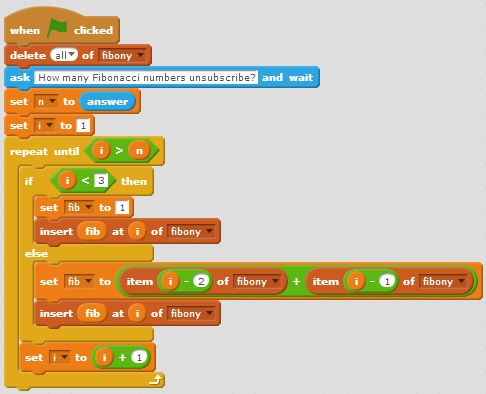
\includegraphics[scale=0.7]{./pics/scratch_fibo_code}
      \caption{Scratch fibonacci code.}
      \label{fig:scratch_fibo_code}
    \end{center}
    \end{subfigure}
    ~
    \begin{subfigure}[b]{0.45\textwidth}
    \begin{center}
      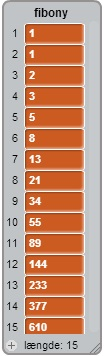
\includegraphics[scale=0.6]{./pics/scratch_fibo_out}
      \caption{Scratch fibonacci output.}
      \label{fig:scratch_fibo_out}
    \end{center}
    \end{subfigure}
    \caption{Code and output for fibonacci numbers.}
    \label{fig:scratch_fibo}
\end{figure}

\subsection{Cups and Ball}
The game of guessing the position of the ball amongst the cups is made with events, as Scratch is able to handle these with blocks. Events happen e.g. when a cup is clicked, cups are cloned, and when the ball is clicked. Code is also attached different sprites, as these work individually to the events. The code blocks for the cups can be seen in \figref{fig:scratch_ball_code1}, and the code blocks for the ball can be seen in \figref{fig:scratch_ball_code2}. A screenshot of the game screen while in a game can be seen in \figref{fig:scratch_ball_out}.

\begin{figure}[h]
  \centering
    \begin{subfigure}[b]{0.45\textwidth}
    \begin{center}
      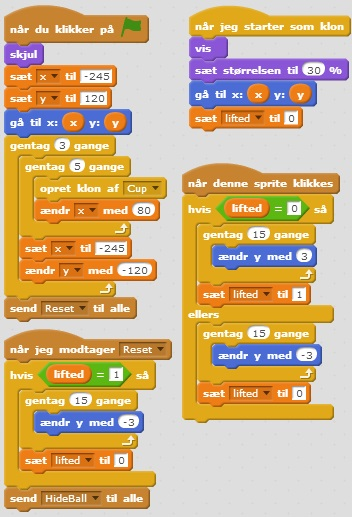
\includegraphics[scale=0.7]{./pics/scratch_ball_code1}
      \caption{Scratch cup code.}
      \label{fig:scratch_ball_code1}
    \end{center}
    \end{subfigure}
    ~
    \begin{subfigure}[b]{0.45\textwidth}
    \begin{center}
      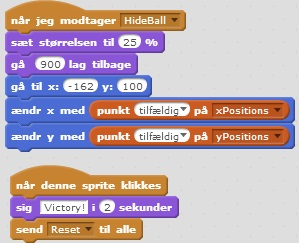
\includegraphics[scale=0.7]{./pics/scratch_ball_code2}
      \caption{Scratch ball code.}
      \label{fig:scratch_ball_code2}
    \end{center}
    \end{subfigure}
    
    \begin{subfigure}[b]{\textwidth}
    \begin{center}
      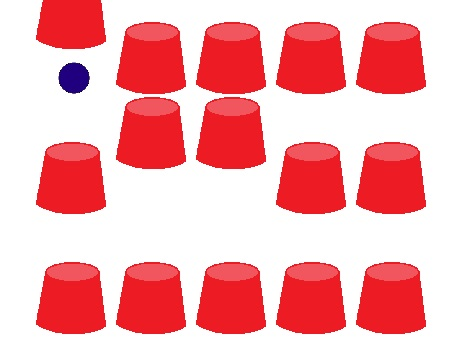
\includegraphics[scale=0.5]{./pics/scratch_ball_out}
      \caption{Scratch Cups and Ball output.}
      \label{fig:scratch_ball_out}
    \end{center}
    \end{subfigure}
    \caption{Code and output for Cups and Ball.}
    \label{fig:scratch_ball}
\end{figure}

\subsection{Hangman}
The Hangman game is made in an imperative manner. As there are many conditions to take into account, the code is rather long, and there is a lot of control structures. The guessing part itself is a big loop, which can be seen in \figref{fig:scratch_hang_code}. On the game screen, a list holds the letters for the word to guess, a list holds all the wrong guesses, and a sprite changes for each wrong guess. An input field is provided for guessing. The game screen can be seen in \figref{fig:scratch_hang_out}.

\begin{figure}[h]
  \centering
    \begin{subfigure}[b]{0.45\textwidth}
    \begin{center}
      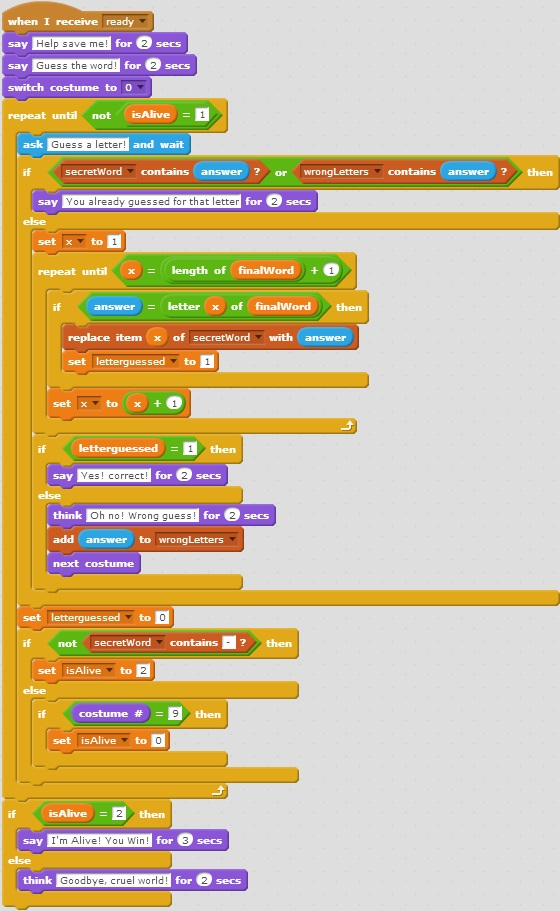
\includegraphics[scale=0.5]{./pics/scratch_hang_code}
      \caption{Scratch Hangman code.}
      \label{fig:scratch_hang_code}
    \end{center}
    \end{subfigure}
    ~
    \begin{subfigure}[b]{0.45\textwidth}
    \begin{center}
      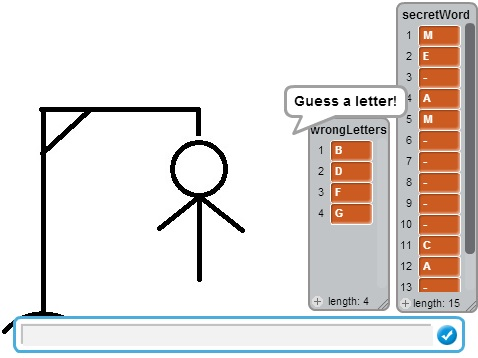
\includegraphics[scale=0.5]{./pics/scratch_hang_out}
      \caption{Scratch Hangman output.}
      \label{fig:scratch_hang_out}
    \end{center}
    \end{subfigure}
    \caption{Code and output for Hangman.}
    \label{fig:scratch_hang}
\end{figure}

\subsection{Criteria Evaluation}

\begin{description}[style=nextline]
\item[Readability] Scratch is known for its great readability, and this shows clearly when reading it. The colored structures clearly show what the different building blocks are doing, and variables are easy to identify. We believe this is a great advantage for novices
\item[Writability] The visual programming style has its pros and cons. It is easy to create simple structures, but it takes too long for an advanced programmer. It is extremely easy to understand how to use scratch, due to the fact that it uses building blocks as arguments.
\item[Observability] Scratch has a live game window, where output is shown when compiling code. Combined with the possibility of double-clicking sets of blocks to compile, the programmer can see the output whenever wanted.
\item[Trialability] The visual environment for Scratch allows close to no syntax errors. Combined with the level of observability, Scratch has great possibility of recovering from errors, as the error is easily found in the game window.
\item[Learnability] Making a game is a good way to capture the attention of children. But to keep them occupied, the process of coding should be intensive in a playful way. Building blocks from the visual style is a way to do it, as building blocks has been proven successful in the context of playing. The lack of proper syntax, however, can be hindering further in the programmer's career. That means the language is great for novice programming, but it comes to a stop.
\item[Reusability] As Scratch is also a minor game engine, it uses 2D sprites for visualization. Each sprite can contain code local to that sprite. As these can be cloned, the code written serves as a blueprint for all instances of the sprite to use. Sadly, it is the only way for Scratch to reuse code.
\item[Pedagogic Value] Scratch makes use of the most basic of concepts, such as variables and control structures. That said, there is a huge leap when moving from Scratch to a non-visual programming language. The missing syntax found in text based programming language can confuse a novice when moving on.
\item[Environment] Scratch has a very friendly environment, with great visibility in the color coding. As novices are not familiar with anything code-related, the naming of structures is meaningful and easy to understand. Navigation can be a bit confusing at first, as it can be hard to know what category a needed block is found in. The control of the blocks can be a bit annoying, as disconnection interlocked blocks does not always go as expected. The game window combined with the block compilation, as mentioned, is a great way of obtaining feedback for trial-and-error.
\item[Documentation] Scratch has an integrated introduction tutorial, which is a great way for novices to learn the language. Furthermore, each building block can be right-clicked to find a documentation page for that specific block. This documentation is easy to read, but is unfortunately only available in English.
\item[Uniformity] The basic concepts used in Scratch do the same as in other languages. However, the naming of the expressions and structures are often different, e.g. Scratch has a \emph{repeat} structure, instead of a \emph{for} structure.
\end{description}